\documentclass[11pt]{ctexart}
\usepackage{tabularx}
\usepackage{array}
\usepackage{bm}
\usepackage{hyperref}
\usepackage{graphicx}
\usepackage{amsmath}
\usepackage{algorithm}
%\usepackage{algorithm2e}
\usepackage{algpseudocode}
\usepackage{fancyhdr}
\pagestyle{fancy}

\hypersetup{hypertex=true,
	colorlinks=true,
	linkcolor=red,
	anchorcolor=blue,
	citecolor=blue}
\fancyhf{}
\chead{\textbf{算法设计与分析}}
\fancyhead[r]{\bfseries\thepage}
\fancyhead[l]{\bfseries\rightmark}
\renewcommand{\headrulewidth}{0.4pt} % 注意不用 \setlength
\renewcommand{\footrulewidth}{0pt}

\floatname{algorithm}{算法}
\renewcommand{\algorithmicrequire}{\textbf{输入:}}
\renewcommand{\algorithmicensure}{\textbf{输出:}}

\begin{titlepage}
	\title{\Huge\textbf{算法设计与分析 作业三}\\}
	\author{\Large\textbf{作者}:吴润泽 \and{\Large\textbf{学号}:181860109}\\
	\\
	\and {\Large\textbf{Email}:\href{mailto:181860109@smail.nju.edu.cn}{181860109@smail.nju.edu.cn}}\\}
	\date{\Large\today}
\end{titlepage}

\begin{document}
	\maketitle
	\tableofcontents
	\newpage
	\section*{SELECTION}
	\markright{SELECTION}
	\addcontentsline{toc}{section}{SELECTION}
	\hypertarget{problem 8.2}{\subsection*{problem 8.2}}
	\markright{problem 8.2}
	\addcontentsline{toc}{subsection}{problem 8.2}
	\paragraph{算法}
	假设有5个数a,b,c,d,e\\
	1.比较a b,将较小者放入a,较大者放入b\\
	2.比较c d,将较小者放入c,较大者放入d\\
	3.比较a c,将较小者放入a,较大者放入c,若a和c发生交换则同时交换b和d,即保证a b和
	c d原有大小关系不变。此时有$a<c<d,a<b$,则a不可能是中位数\\
	4.比较b e,将较小者放入b,较大者放入e\\
	5.比较b c,将较小者放入b,较大者放入c,若b和c发生交换则同时交换d和e,即保证b e和
	c d原有大小关系不变。此时有$b<c<d,b<e$,则b不可能是中位数\\
	6.比较c e,\hspace{5pt}将较小者放入c,较大者放入e,此时有$c<d<e$,且$c>b,c>a$,即c就是中位数。\\
	\begin{figure}[h]
		\centering
		\caption{决策树}
		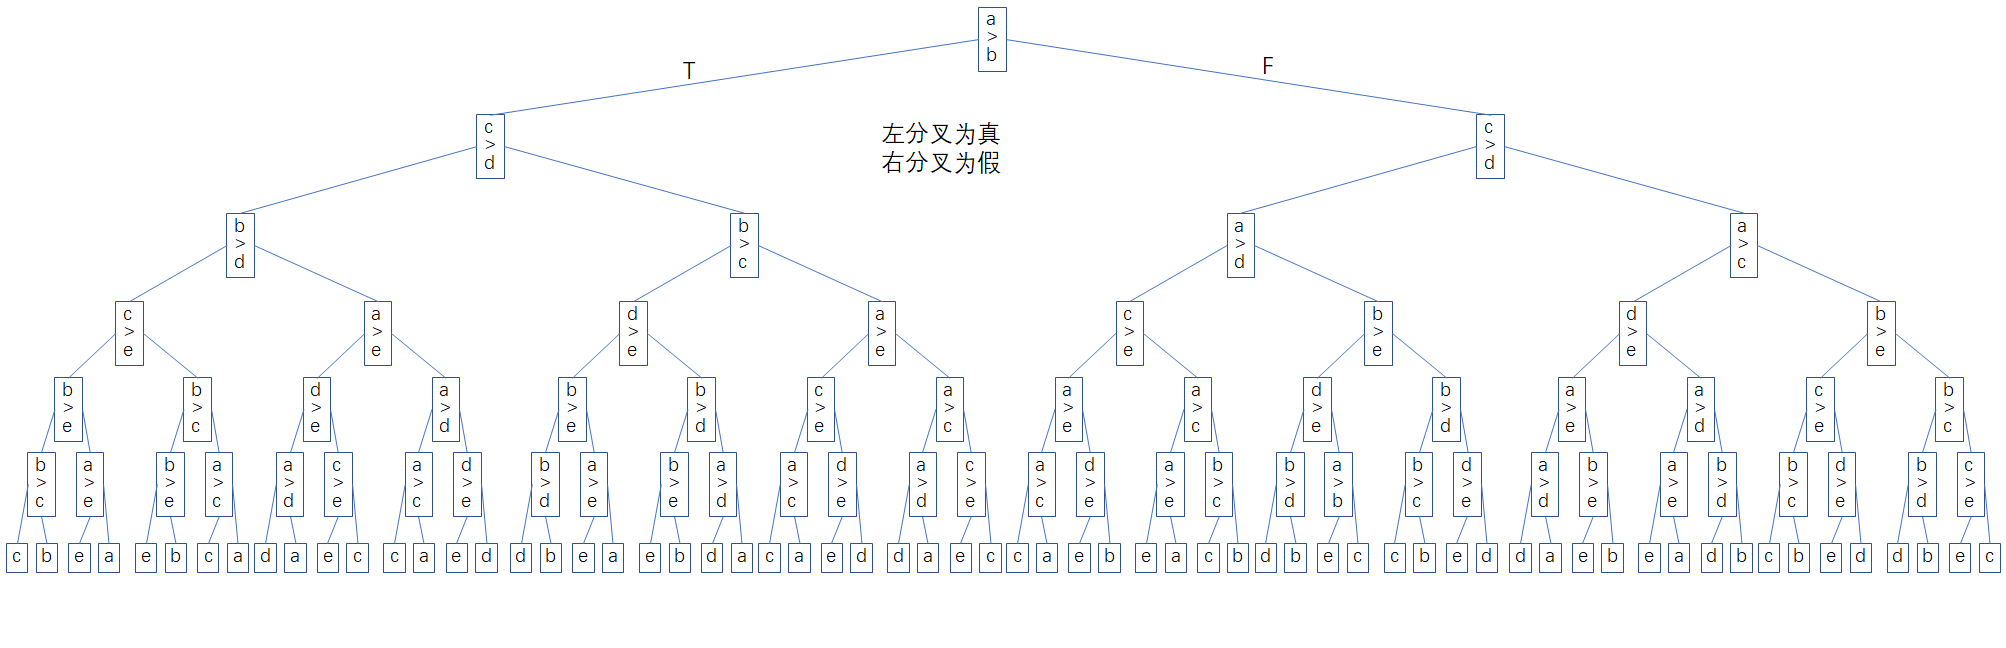
\includegraphics[height=220pt,width=450pt]{tree.png}

	\end{figure}

	\newpage
	\hypertarget{problem 8.4}{\subsection*{problem 8.4}}
	\markright{problem 8.4}
	\addcontentsline{toc}{subsection}{problem 8.4}
	\paragraph{算法}
	设数组array元素个数为n,不妨设n为奇数,阶为k的元素为m;\\
	1. 当k等于$\frac{n+1}{2}$时,直接调用算法A,即可找到m;\\
	2. 当k小于$\frac{n+1}{2}$时,遍历数组array,记录其元素最小值为min,对于原数组array,有$n-k$个元素大于m,$k-1$个元素小于m。\\
	3. 开辟新数组temp,将前$n-2k+1$个元素值赋为min-1,并将array的n个元素放入其后。
	则数组temp中有$n-k$个元素大于m,$n-k$个元素小于m。因此m为temp中位数,调用算法A,即可找到m。\\
	4. 当k大于$\frac{n+1}{2}$时,同理记录其元素最大值为max,开辟数组temp,在数组temp中前$2k-n-1$个赋值为max+1。同样使得m变为temp中位数,调用算法A,即可找到m。\\
	\label{Kth-find算法}
	$\begin{aligned}
	\hline
	&\textbf{算法1 }KthFind\text{ 算法}\\
	\hline
	&1.\textbf{Function}\ {KthFind}\ (array,n,k)\\
	&2.\hspace*{20pt}\textbf{if }k==\frac{n+1}{2}\textbf{ return }A(array,n)\\
	&3.\hspace*{20pt}min\_num:= min(array,n),max\_num:= max(array,n)\\
	&4.\hspace*{20pt}Let\ temB[1...2n]\ be\ new\ array.\\
	&5.\hspace*{20pt}\textbf{for}\ i:= 1\ to\ n\ \textbf{do}\\
	&6.\hspace*{40pt}temB[i]:=A[i]\\
	&7.\hspace*{20pt}\textbf{if }k<\frac{n+1}{2} \textbf{ then}\\
	&8.\hspace*{40pt}\textbf{for}\ i:= 1\ to\ n-2k+1\ \textbf{do}\\
	&9.\hspace*{60pt}temB[i+n]:= min\_num-1\\
	&10.\hspace*{35pt}\textbf{return }A(temB,2n-2k+1)\\
	&11.\hspace*{15pt}\textbf{if }k>\frac{n+1}{2} \textbf{ then}\\
	&12.\hspace*{35pt}\textbf{for}\ i:= 1\ to\ 2k-n-1\ \textbf{do}\\
	&13.\hspace*{55pt}temB[i+n]:= max\_num-1\\
	&14.\hspace*{35pt}\textbf{return }A(temB,2k-1)\\
	\hline
	\end{aligned}
	$

	\paragraph{时间复杂度}寻找最值和开辟新数组的时间复杂度为$O(n)$,添加的元素个数最多为$n-1$个,数组的规模仍为$O(n)$,而找中位数算法A,时间复杂度为$O(n)$,因此总的时间复杂度仍为线性。

	\subsection*{problem 8.5}
	\markright{problem 8.5}
	\addcontentsline{toc}{subsection}{problem 8.5}
	\subsubsection*{(1)}使用归并排序进行降序排列,排序结果前k个元素即为所求。\\
	归并排序时间复杂度为$O(n\log n)$,输出复杂度为$O(k)$,总时间复杂度为$O(n\log n)$.\\
	$\begin{aligned}
	\hline
	&1.\textbf{Function}\ {KthOrder1}\ (array,n,k)\\
	&2.\hspace*{20pt}\text{对原数组使用归并排序,并按照升序排列}\\
	&3.\hspace*{20pt}\textbf{for}\ i:= 1\ to\ k\ \textbf{do}\\
	&4.\hspace*{40pt}res.add(array[i])\\
	&5.\hspace*{20pt}\textbf{return }res\\
	\hline
	\end{aligned}
	$
	\subsubsection*{(2)}根据原数组建立最大堆,最大堆堆顶存储当前堆的最大值,则弹出堆顶元素k次,k个元素即为所求。\\
	根据已有序列建堆的时间复杂度为$O(n)$,弹出堆顶元素k次,每次修复堆时间复杂度为$O(\log n)$,则总的时间复杂度为$O(n+k\log n)$.\\
	$\begin{aligned}
	\hline
	&1.\textbf{Function}\ {KthOrder2}\ (array,n,k)\\
	&2.\hspace*{20pt}\text{根据原数组进行建堆,得到最大堆为heap}\\
	&3.\hspace*{20pt}\textbf{for}\ i:= 1\ to\ k\ \textbf{do}\\
	&4.\hspace*{40pt}res.add(heap.top())\\
	&5.\hspace*{40pt}heap.pop()\verb|\\|\text{弹出堆顶元素,并修复}\\
	&6.\hspace*{20pt}\textbf{return }res\\
	\hline
	\end{aligned}
	$
	\hypertarget{problem 8.5(3)}{\subsubsection*{(3)}}
	利用 \hyperlink{problem 8.4}{problem 8.4} 中 \hyperref[Kth-find算法]{Kth-find算法} ,找到原数组中的第k+1大元素m。遍历原数组,找到其中大于m的元素加入结果数组res。 对res使用归并排序,升序排列,得到res即为所求。\\
	找第k+1大,遍历原数组为线性时间$O(n)$,对res归并排序$O(k\log k)$,总时间复杂度为$O(n+k\log k)$.\\
	$\begin{aligned}
	\hline
	&1.\textbf{Function}\ {KthOrder3}\ (array,n,k)\\
	&2.\hspace*{20pt}m:=KthFind(array,n,k+1)\verb|\\找到数组第k+1大元素|\\
	&3.\hspace*{20pt}\textbf{for}\ i:= 1\ to\ n\ \textbf{do}\\
	&4.\hspace*{40pt}\textbf{if }array[i]>m \textbf{ do } res.add(array[i])\\
	&5.\hspace*{20pt}\text{对res数组使用归并排序,并按照升序排列}\\
	&6.\hspace*{20pt}\textbf{return }res\\
	\hline
	\end{aligned}
	$
	\subsection*{problem 8.6}
	\markright{problem 8.6}
	\addcontentsline{toc}{subsection}{problem 8.6}
	\subsubsection*{(1)}使用归并排序进行排列时间复杂度为$O(n\log n)$,遍历中位数M左右两侧元素,与M差值最小的加入res,并移动对应侧指针,直至res个数为k即可。总时间复杂度为$O(n\log n+k)$.\\
	$\begin{aligned}
	\hline
	&1.\textbf{Function}\ {KthNear1}\ (array,n,k)\\
	&2.\hspace*{20pt}\text{对原数组使用归并排序}\\
	&3.\hspace*{20pt}l:=\frac{n+1}{2}-1,\ r:=\frac{n+1}{2}+1\\
	&4.\hspace*{20pt}\textbf{for}\ i:= 1\ to\ k\ \textbf{do}\\
	&5.\hspace*{40pt}\textbf{if }array[l]+array[r]>2M \textbf{ do } res.add(array[r++])\\
	&6.\hspace*{40pt}\textbf{else }res.add(array[l--])\\
	&7.\hspace*{20pt}\textbf{return }res\\
	\hline
	\end{aligned}
	$
	\subsubsection*{(2)}利用 \hyperlink{problem 8.4}{problem8.4} 中的查找中位数算法,得到中位数为M,时间复杂度为$O(n)$。
	\hspace*{20pt}将原数组分为大于M和小于M的两数组L,S,时间复杂度为$O(n)$。
	\hspace*{20pt}与 \hyperlink{problem 8.5(3)}{problem 8.5(3)} 同样思想,找到L的前k小(查找第k+1小,即第n-k-1大)LK和S的前k大元素SK,时间复杂度为$O(k)$。对LK进行归并排序按照升序排列,对SK进行归并排序按照降序排列,时间复杂度为$O(k\log k)$。
	之后遍历LK和SK找到与M最接近的K个元素即可。\\
	$\begin{aligned}
	\hline
	&1.\textbf{Function}\ {KthNear2}\ (array,n,k)\\
	&2.\hspace*{20pt}M:=A(array,n)\verb|\\|\text{找到中位数M}\\
	&3.\hspace*{20pt}\text{划分原数组为大于M和小于M两部分:L[1..n1],S[1..n2]}\\
	&4.\hspace*{20pt}large:=KthFind(L,n1,n1-k-1)\verb|\\找到L数组第k+1小元素|\\
	&5.\hspace*{20pt}small:=KthFind(S,n2,k+1)\verb|\\找到L数组第k+1大元素|\\
	&6.\hspace*{20pt}\text{找到L数组小于large的k个元素,并升序排列,得到LK}\\
	&7.\hspace*{20pt}\text{找到S数组大于small的k个元素,并降序排列,得到SK}\\
	&8.\hspace*{20pt}l:=0,\ r:=0\\
	&9.\hspace*{20pt}\textbf{for}\ i:= 1\ to\ k\ \textbf{do}\\
	&10.\hspace*{35pt}\textbf{if }LK[l]+SK[r]>2M \textbf{ do } res.add(SK[r++])\\
	&11.\hspace*{15pt}\textbf{else }res.add(LK[l--])\\
	&12.\hspace*{15pt}\textbf{return }res\\
	\hline
	\end{aligned}
	$
	\newpage
	\subsection*{problem 8.8}
	\markright{problem 8.8}
	\addcontentsline{toc}{subsection}{problem 8.8}
	\paragraph{算法设计}
	 使用两个堆,大根堆q1维护较小值,小根堆维护较大值,令大根堆q2元素个数为$m$,小根堆元素个数为$n$:\\
	 \hspace*{20pt}使得小根堆的堆顶是较大数中最小的,大根堆的堆顶是较小数中最大的;\\
	 \hspace*{20pt}将大于大根堆堆顶的数放小根堆,小于等于大根堆堆顶的数放大根堆;\\
	 对于大根堆的堆顶元素,有$n$个元素比该元素大,$m-1$个元素比该元素小;\\
	 对于小根堆的堆顶元素,有$m$个元素比该元素小, $n-1$个元素比该元素大;\\
	在维护$|m-n| \leq 1$之后,当$m=n$时,两堆顶元素均为中位数,当$m\ne n$时,元素个数较多的堆顶元素即为当前中位数;\\
	易知插入和删除的时间复杂度均为$O(\log n)$,查找中值为常数。\\
	$\begin{aligned}
	&\textbf{查找中值}\\
	\hline
	&1.\hspace*{20pt}\textbf{if }(q1.size()+q2.size())\%2==1\textbf{ then }\\
	&2.\hspace*{40pt}\textbf{if }q1.size()>q2.size()\textbf{ do }mid:=q1.top()\\
	&3.\hspace*{40pt}\textbf{else } mid:=q2.top()\\
	&4.\hspace*{20pt}\textbf{else } mid:=(q1.top+q2.top())/2\\
	\hline
	\end{aligned}\\
	$$
	\begin{aligned}
	&\textbf{插入操作}\\
	\hline
	&1.\hspace*{20pt}\textbf{if }input > q1.top()\textbf{ do }q2.push(input)\\
	&2.\hspace*{20pt}\textbf{else }myq1.push(input)\verb|\\|\text{大根堆放较小数,小根堆放较大数}\\
	&3.\hspace*{20pt}\textbf{while }|q1.size()-q2.size()|>1\textbf{ do}\\
	&4.\hspace*{40pt}\textbf{if }q1.size()>q2.size()\textbf{ do }q2.push(q1.pop())\\
	&4.\hspace*{40pt}\textbf{else } q1.push(q2.pop())\\
	\hline
	\end{aligned}\\
	$
	$
	\begin{aligned}
	&\textbf{删除操作}\\
	\hline
	&1.\hspace*{20pt}\textbf{if }(q1.size()+q2.size())\%2==1\textbf{ then }\\
	&2.\hspace*{40pt}\textbf{if }q1.size()>q2.size()\textbf{ do }q1.pop()\\
	&3.\hspace*{40pt}\textbf{else }q2.pop()\\
	&4.\hspace*{20pt}\textbf{else }q2.pop()\verb|\\|\text{当为偶数时任意弹出一个}\\
	\hline
	\end{aligned}
	$
	\newpage
	\subsection*{problem 8.9}
	\markright{problem 8.9}
	\addcontentsline{toc}{subsection}{problem 8.9}
	\subsubsection*{(1)}
	对中位数$x_k$,设n为奇数,有$\frac{n+1}{2}-1$个元素小于$x_k$,$\frac{n+1}{2}-1$个元素大于$x_k$,则$\sum_{x_i>x_k}\frac{1}{n}=\sum_{x_i<x_k}\frac{1}{n}=\frac{1}{2}-\frac{1}{2n}<\frac{1}{2}.$对n为偶数,同样成立。
	\subsubsection*{(2)}
	建立以(w,x)为元素的结构体数组ori,w为权重,x为其对应下标。对其进行归并排序,时间复杂度为$O(n\log n)$。遍历ori,对权重进行累加,当权重和大于$\frac{1}{2}$时,对应结构体元素的x即为加权中位数,时间复杂度为$O(n)$。因此总的时间复杂度为$O(n\log n)$。\\
	$\begin{aligned}
	\hline
	&1.\textbf{Function}\ {WeightMid1}\ (ori,n)\\
	&2.\hspace*{20pt}\text{对结构体数组ori使用归并排序}\\
	&3.\hspace*{20pt}cur\_weight:=0\verb|\\|\text{当前权重}\\
	&4.\hspace*{20pt}\textbf{for}\ i:= 1\ to\ n\ \textbf{do}\\
	&5.\hspace*{40pt}\textbf{if }cur\_weight+ori[i].w>\frac{1}{2} \textbf{ do }\\ 	&6.\hspace*{60pt}\textbf{return }ori[i].x\\
	&7.\hspace*{40pt}\textbf{else }\verb|\\|\text{更新权重和权重}\\
	&8.\hspace*{60pt}cur\_weight:=cur\_weight+ori[i].w\\
	\hline
	\end{aligned}
	$
	\subsubsection*{(3)}
	\paragraph{参考BFRPTR算法}假设划分的权值和为tar,初始$tar=\frac{1}{2}$\\
	1. 将所有元素分成$\lceil\frac{n}{5}\rceil$组,每组5个元素(最后一组可能不足5个元素)\\
	2. 寻找$\lceil\frac{n}{5}\rceil$组中每一组的中位数,可对每一组进行排序\\
	3. 对于找出的$\lceil\frac{n}{5}\rceil$个中位数递归进行1,2直到剩下一个数即为中位数,记为m\\
	4. 基于m对元素进行划分,假设有x个元素小于m,n-x-1个元素大于m\\
	5. 计算x个元素的权值和T,若权值和T=tar,则m为加权平均数\\
	6. 若权值和T>tar,则在x个元素中递归寻找中位数,tar值不变\\
	7. 若权值和T<tar,则在n-x-1个元素中递归寻找中位数,tar=tar-T\\
	8. 时间复杂度$T(n)=T(n/5)+T(7n/10)+O(n)=\Theta(n)$,满足要求。\\
	\textbf{算法实现}\\
	$
	\begin{aligned}
	\hline
	&1.\textbf{Function}\ {Partion}\ (ori,l,r)\verb|\\|\text{根据ori[l]进行划分}\\
	&2.\hspace*{20pt}i:=l,j:=r,pivot:=ori[l]\\
	&3.\hspace*{20pt}\textbf{while }i<j:\\
	&4.\hspace*{40pt}\textbf{while }ori[j].w<=mid.w\textbf{ and }i<j:\ ori[i]:=ori[--j]\\
	&5.\hspace*{40pt}\textbf{while }ori[i].w>=mid.w\textbf{ and }i<j:\ ori[j]:=ori[--i]\\
	&6.\hspace*{20pt}ori[i]:=pivot\\
	&7.\hspace*{20pt}\textbf{return }i\\
	\hline
	\end{aligned}\\
	$
	$
	\begin{aligned}
	\hline
	&1.\textbf{Function}\ {FindMid}\ (ori,l,r)\verb|\\|\text{寻找中位数的中位数}\\
	&2.\hspace*{20pt}n:=0\verb|\\|\text{计算中位数个数}\\
	&3.\hspace*{20pt}\textbf{for}\ (i:= l;r-5;i+=5)\\
	&4.\hspace*{40pt}sort(ori,i,i+4)\verb|\\|\text{对5个数进行排序}\\
	&5.\hspace*{40pt}n:=i-l,\ swap(ori[l+n/5],ori[i+2])\verb|\\|\text{将该组中位数放在数组头}\\
	&6.\hspace*{20pt}\verb|\\|\text{相同办法处理数组剩余元素}\\
	&7.\hspace*{20pt}\textbf{if }n/5==l\textbf{ return }ori[l]\\
	&8.\hspace*{20pt}\textbf{return }FindMid(ori,l,l+n/5)\\
	\end{aligned}
	$
	$
	\begin{aligned}
	\hline
	&1.\textbf{Function}\ {BFPTR}\ (ori,l,r,tar)\\
	&2.\hspace*{20pt}FindMin(ori,l,r)\verb|\\|\text{寻找权值中位数m和其下标x}\\
	&3.\hspace*{20pt}pos:=Partion(ori,l,r)\verb|\\|\text{根据m来划分ori为小于和大于m两部分}\\
	&4.\hspace*{20pt}cur:=0\\
	&5.\hspace*{20pt}\textbf{for}\ i:= l\ to\ pos\ \textbf{do}
	\verb|  \\|\text{计算l-pos的权重}\\
	&6.\hspace*{40pt}cur:=cur+ori[i].w\\
	&7.\hspace*{20pt}\textbf{if }cur==tar\textbf{ return }ori[i].x\\
	&8.\hspace*{20pt}\textbf{elif }cur<tar\textbf{ return }BFPTR(ori,pos+1,r,tar-cur)\\
	&9.\hspace*{20pt}\textbf{else return }BFPTR(ori,0,pos-1,tar)\\
	\hline
	\end{aligned}
	$
	\newpage
	\section*{SEARCH}
	\markright{SEARCH}
	\addcontentsline{toc}{section}{SEARCH}
	\subsection*{problem 9.4}
	\markright{problem 9.4}
	\addcontentsline{toc}{subsection}{problem 9.4}
	\paragraph{引理9.1}证明:\\
	\hypertarget{9.1 (1)}{
	\textbf{(1)数学归纳法}}\\
	当h=0时,内部节点有0个,成立\\
	假设当h=n-1时,内部黑色节点个数$x\geq 2^{n-1}-1$个\\
	当h=n时,为满足每条路径黑色深度相等,即最底层外部结点全部替换为黑色内部节点,增加$2^{n-1}$个黑色内部节点,所以$x+2^{n-1}\geq2^{n}-1$,成立。\\
	\hypertarget{9.1 (2)}{\textbf{(2)}}\\
	内部节点最多时,任何一条路径上均为黑红节点交替,黑色节点位于首尾共h+1个,因此每条路径的红色节点为h个,因此树的高度(抛去外部节点)为2h。且满足完美二叉树性质,内部节点个数为$2^{2h}-1=4^h-1$,成立。\\
	\hypertarget{9.1 (2)}{\textbf{(3)反证法}}\\
	假设存在黑色节点的普通高度超过其黑色高度的2倍,设其黑色高度为k,则总高度超过2k,亦即红色结点个数超过k,则必然存在红色结点在路径上连续,与定义相矛盾,故任何黑色节点的普通高度至少是其黑色高度2倍。
	\paragraph{引理9.2}证明:\\
	\textbf{(1)}\\
	由红黑树定义,$ARB_h$可看作由红色根节点和两棵$RB_{h-1}$树(原为子结点的黑色节点变为根节点)组成。
	由\hyperlink{9.1 (1)}{引理9.1(1)}$RB_{h-1}$内部黑色节点至少为$2^{h-1}-1$,因此$ARB_h$内部黑色节点至少为$2(2^{h-1}-1)=2^h-2$,成立。\\
	\textbf{(2)}\\
	同样利用$ARB_h$由红色根节点和两棵$RB_{h-1}$树组成。
	由\hyperlink{9.1 (2)}{引理9.1(2)}$RB_{h-1}$内部节点最多为$4^{h-1}-1$,因此$ARB_h$内部节点最多为$2(4^{h-1}-1)+1=\frac{4^h}{2}-1$,成立。\\
	\textbf{(3)反证法}\\
	与\hyperlink{9.1 (3)}{引理9.1(3)}证法相同,
	假设存在黑色节点的普通高度超过其黑色高度的2倍,则必然存在红色结点在路径上连续,与定义相矛盾,故任何黑色节点的普通高度至少是其黑色高度2倍。
	\subsection*{problem 9.6}
	\markright{problem 9.6}
	\addcontentsline{toc}{subsection}{problem 9.6}
	\paragraph{算法设计}
	采取二分查找的方法,设访问的元素为$A[i]$,$res$存放结果,$l,r$记录查找区间;\\
	若$A[i]=i$,说明$1-i$没有缺少元素,则向右半边递归查找;\\
	若$A[i]>i$,说明$1-i$已经缺少元素,更新$res:=i$,向左半边递归查找;\\
	当$l>r$时,递归结束返回res即可。\\
	
	\par
	\noindent
	\textbf{算法实现}
	\\
	$\begin{aligned}
	\hline
	&\textbf{算法1 }FindLeastNum\text{ 算法}\\
	\hline
	&1.\textbf{Function}\ FindLeastNum\ (A[1\cdots n])\\
	&2.\hspace*{20pt}l:=1,r:=n\\
	&3.\hspace*{20pt}\textbf{while }l\leq r\textbf{ do}\\
	&4.\hspace*{40pt}mid:=(r-l)/2+l\\
	&5.\hspace*{40pt}\textbf{if }A[mid]>i\textbf{ then}\\
	&6.\hspace*{60pt}res:=i,r:=mid-1\\
	&7.\hspace*{40pt}\textbf{else }\\
	&8.\hspace*{60pt}l=mid+1\\
	&9.\hspace*{20pt}\textbf{return }res\\
	\hline
	\end{aligned}
	$
	\paragraph{时间复杂度}较易分析,每次缩小区间为原来的一半,因此查找时间复杂度为$O(\log n)$。
	\newpage
	\subsection*{problem 9.8}
	\markright{problem 9.8}
	\addcontentsline{toc}{subsection}{problem 9.8}
	\paragraph{算法设计}矩阵为A,当前行为row,当前列为col,待查找元素为tar\\
	1. 从右上角开始遍历,当$A[row][col]>tar$,说明不在这一列中,col减1;\\
	2. 当$A[row][col]<tar$,说明不在这一行中,row加1;\\
	3. 当$A[row][col]=tar$,查找成功。否则当查找结束,返回查找失败。\\
	\par
	\noindent
	\textbf{算法实现}
	\\
	$\begin{aligned}
	\hline
	&\textbf{算法2 }SearchMatrix\text{ 算法}\\
	\hline
	&1.\textbf{Function}\ SearchMatrix\ (A[1\cdots m][1\cdots n],tar)\\
	&2.\hspace*{20pt}row:=1,col:=n\\
	&3.\hspace*{20pt}\textbf{while }row\leq n\textbf{ and }col\geq 0\textbf{ do}\\
	&4.\hspace*{40pt}\textbf{if }(A[row][col]>tar)\ col--\\
	&5.\hspace*{40pt}\textbf{if }(A[row][col]<tar)\ row++\\
	&6.\hspace*{40pt}\textbf{else }\textbf{return }true\\
	&7.\hspace*{20pt}\textbf{return }false\\
	\hline
	\end{aligned}
	$
	\paragraph{最坏情况}在每次比较中都可以排除一行或者一列,共有$(m+n)$行列,当行或列减到0查找失败,因此最坏情况下需要比较$m+n-1$次。
	\newpage
	\subsection*{problem 9.12}
	\markright{problem 9.12}
	\addcontentsline{toc}{subsection}{problem 9.12}
	\subsection*{(1)}
	\paragraph{算法设计}
		采取二分查找方法,设访问的元素为$A[mid]$,$l,r$记录区间;\\
	1. 若$A[mid-1]\leq A[mid]\leq A[mid+1]$,找到一个局部最小元素返回即可。\\
	2. 若$A[mid]>A[mid+1]$,同时$A[n-1]\leq A[n]$,$mid-n$区间满足原数组性质,则向右半部分递归查找。\\
	3. 当$A[mid-1]<A[mid]$时,同理向左半部分递归查找。\\
	$\begin{aligned}
	\hline
	&\textbf{算法2 }SearchNeighborMin\text{ 算法}\\
	\hline
	&1.\textbf{Function}\ SearchNeighborMin\ (A[1\cdots m][1\cdots n])\\
	&2.\hspace*{20pt}l:=1,r:=n\\
	&3.\hspace*{20pt}\textbf{while }l\leq r\textbf{ do}\\
	&4.\hspace*{40pt}mid:=(r-l)/2+l\\
	&5.\hspace*{40pt}\textbf{if }(A[mid]>A[mid-1])\ r:=mid-1\\
	&6.\hspace*{40pt}\textbf{elif }A[mid]>A[mid+1]\ l:=mid+1\\
	&7.\hspace*{40pt}\textbf{else }\textbf{return }mid\\
	\hline
	\end{aligned}
	$
	\subsection*{(2)证明}
	数组中一定存在最小值,当最小值不为边界时,即满足$A[i+1]\geq A[i]\leq A[i-1]$,即一定是局部最小元素。\\
	当最小值为边界元素时,又因为满足$A[1]\geq A[2],A[n-1]\leq A[n]$则:\\
	1. 当$A[1]$为最小值时,一定有$A[1]=A[2]\leq A[3]$,$A[2]$为局部最小元素\\
	2. 当$A[n]$为最小值时,一定有$A[n-2]\geq A[n-1]= A[n]$,$A[n-1]$为局部最小元素。
	故数组中至少存在一个局部最小元素。
	\newpage
	\section*{HASH}
	\markright{HASH}
	\addcontentsline{toc}{section}{HASH}
	\subsection*{problem E1}
	\markright{problem E1}
	\addcontentsline{toc}{subsection}{problem E1}
	\subsection*{(1)} 
	\paragraph{闭散列}设其负载因子为$\alpha,\alpha\ \in\{0.25,0.5,1.0,2.0\}$,其初始空位为$h_C$,则链表节点个数为$\alpha h_C$,因此其空间消耗为$2\alpha h_C$。
	因此当$\alpha$分别为0.25,0.5,1.0,2.0时,闭散列空间消耗分别为:
	$\left\{
	\begin{aligned}
	&\textbf{0.25}: 0.5h_C\\
	&\textbf{0.5}: h_C\\
	&\textbf{1.0}: 2h_C\\
	&\textbf{2.0}: 4h_C\\
	\end{aligned}
	\right.
	$
	\paragraph{开散列}设其负载因子为$\alpha_1$,则其关键字个数为$\alpha_1 h_C$,其空间消耗为$\alpha_1 h_C$,
	即$\alpha_1 h_C=2\alpha h_C\Rightarrow \alpha_1=2\alpha$,则当闭散列负载因子$\alpha$分别为0.25,0.5,1.0,2.0时,开散列对应的负载因子$\alpha_1$分别为:$$\textbf{0.5,1,2,4}.$$
	
	\subsection*{(2)}
	\paragraph{闭散列}同理其空间消耗为$5\alpha h_C$。
	因此当$\alpha$分别为0.25,0.5,1.0,2.0时,闭散列空间消耗分别为:
	$\left\{
	\begin{aligned}
	&\textbf{0.25}: 1.25h_C\\
	&\textbf{0.5}: 2.5h_C\\
	&\textbf{1.0}: 5h_C\\
	&\textbf{2.0}: 10h_C\\
	\end{aligned}
	\right.
	$
	\paragraph{开散列}同理其空间消耗为$4\alpha_1 h_C$,
	即$4\alpha_1 h_C=5\alpha h_C\Rightarrow \alpha_1=\frac{5}{4}\alpha$,开散列对应的负载因子$\alpha_1$分别为:$$\textbf{ 0.3125,0.625,1.25,2.5}.$$

	\subsection*{problem E2}
	\markright{problem E2}
	\addcontentsline{toc}{subsection}{problem E2}
	\paragraph{平摊分析} 假设输入的规模为n,由数组i的大小为$2^i$可知,最后一个不为空的数组的下标$x=\lfloor\log n\rfloor$,即每个元素插入后最多下沉$\lfloor\log n\rfloor$次。\\
	对于插入,其$Actual\ Cost=1$,记$Accounting Cost=\log n$\\
	当元素下降至第$m$层时,其总的下降消耗即为从第0层下降至第$m$层,即元素的消耗不超过$\lfloor\log n\rfloor$。\\

	\begin{table}[h]

	\begin{tabular}{|c|c|c|c|c}
		\hline
		\textbf{操作}& \textbf{Amortized Cost} & \textbf{Actual Cost} & \textbf{Accounting Cost}\\
		\hline
		Insert & $1+\log n$ & 1 & $\log n$ \\
		\hline
	\end{tabular}
	\end{table}
	\par
	因此插入n次的总的消耗为$n(1+\log n)=n+n\log n$,则插入n次的时间复杂度为$O(n\log n)$。
	\newpage
	\subsection*{problem E3}
	\markright{problem E3}
	\addcontentsline{toc}{subsection}{problem E3}
	\subsection*{(1)} 设两个栈为A,B\\
	\textbf{Enqueue}将新元素压入B中;\\
	\textbf{Dequeue}如果A不为空,从A中弹出元素;如果A为空,B中所有元素依次出栈并压入A中,即使得A中弹栈顺序变为原始序列输入顺序.
	\subsection*{(2)}
	比较简单的Dequeue(即A不为空)的$Actual\ Cost=1+1=2$,即判断empty和pop;\\
	\hspace*{20pt}而比较复杂的Dequeue,设B中元素个数为t,则$Actual\ Cost=1+2t+1=2t+2$,判断empty,B中pop t个,向A push t个,最后A pop。\\
	\hspace*{20pt}对于Enqueue,$Actual\ Cost=1$,记$Accounting\ Cost$为3,即之后的判空,pop和push的代价。\\
	\hspace*{20pt}则对于复杂的Dequeue的$Accounting\ Cost=-3\times t=-3t$,即减去在Enqueue中的$Accounting\ Cost$。\\
	\begin{table}[h]
	
		\begin{tabular}{|c|c|c|c|c}
			\hline
			\textbf{操作}& \textbf{Amortized Cost} & \textbf{Actual Cost} & \textbf{Accounting Cost}\\
			\hline
			Enqueue & $4$ & 1 & $3$ \\
			\hline
			Dequeue(easy) & $2$ & 2 & $0$ \\
			\hline
			Dequeue(diff) & $2$ & $3t+2$ & $-3t$ \\
			\hline
		\end{tabular}
\end{table}
	\par 即两种情况下Dequeue的消耗相同,若规模为n,入队出队平摊分析法得到的时间复杂度为:
	$$Enqueue(n)+Dequeue(n)=O(6n).$$
\end{document}